\chapter{Probl\`emes de chocs des particules}

\section{D\'esint\'egrations de deux particules}

\subsection{Relation entre $\theta_{1}$ et $\theta_{2}$ dans <<~l~>>}

L'objectif ici est d'obtenir la relation entre $\theta_{1}$ et $\theta_{2}$ dans le r\'ef\'erentiel <<~l~>> dans le cadre de la d\'esint\'egration d'une particule de vitesse initiale $\vec{V}$ en deux particules r\'esultantes de masse respective $m_{1}$ et $m_{2}$. Dans le r\'ef\'erentiel <<~c~>>, le centre d'inertie est immobile, aussi :
\be
	\vec{R} = \dfrac{m_{1}\vec{r}_{10} + m_{2}\vec{r}_{20}}{m_{1} + m_{2}}
\ee
donne :
\bea
	\dfrac{\mathrm{d}\vec{R}}{\mathrm{dt}} & = & \vec{0} \nonumber \\
	m_{1}\vec{v}_{10} + m_{2}\vec{v}_{20} & = & \vec{0}
\eea
qui permet d'\'ecrire :
\bea
	m_{1}\lVert \vec{v}_{10} \rVert & = & m_{2}\lVert \vec{v}_{20} \rVert \nonumber \\
	\dfrac{m_{1}}{m_{2}} & = & \dfrac{v_{20}}{v_{10}}
\eea
mais \'egalement en utilisant le r\'esultat pr\'ec\'edent :
\bea
	m_{1}^{2}v_{10}^{2} + m_{2}^{2}v_{20}^{2} + 2 m_{1}m_{2}v_{10}v_{20}\cos(\theta_{10} + \theta_{20}) & = & 0 \nonumber \\
	m_{1}^{2}v_{10}^{2} + m_{1}^{2}v_{10}^{2} + 2 m_{1}^{2}v_{10}^{2}\cos(\theta_{10} + \theta_{20}) & = & 0 \nonumber \\
	\cos(\theta_{10} + \theta_{20}) & = & -1 \nonumber \\
	\theta_{10} + \theta_{20} & = & \pi
\eea

Les particules r\'esultantes n'interagissant pas l'une sur l'autre, la relation (\ref{EQ:16_5}) est applicable \`a l'une et l'autre telle que :
\bea
	\tan\theta_{1} = \dfrac{v_{10}\sin\theta_{10}}{V + v_{10}\cos\theta_{10}} & \text{ et } & \tan\theta_{2} = \dfrac{v_{20}\sin\theta_{20}}{V + v_{20}\cos\theta_{20}} \nonumber \\
	v_{10}\cos\theta_{10} + V = \dfrac{v_{10}\sin\theta_{10}}{\tan\theta_{1}} & \text{ et } & v_{20}\cos\theta_{20} + V = \dfrac{v_{20}\sin\theta_{20}}{\tan\theta_{2}} \nonumber \\
	V + v_{10}\cos\theta_{10} = \dfrac{v_{10}\sin\theta_{10}}{\tan\theta_{1}} & \text{ et } & V - v_{20}\cos\theta_{10} = \dfrac{v_{20}\sin\theta_{10}}{\tan\theta_{2}}
\eea
La premi\`ere relation permet d'\'ecrire :
\be
	\cos\theta_{10} = \dfrac{\sin\theta_{10}}{\tan\theta_{1}} - \dfrac{V}{v_{10}}
\ee
qui, inject\'ee dans la seconde :
\bea
	V - \dfrac{v_{20}\sin\theta_{10}}{\tan\theta_{1}} + \dfrac{v_{20}V}{v_{10}} & = & \dfrac{v_{20}\sin\theta_{10}}{\tan\theta_{2}} \nonumber \\
	\left(1 + \dfrac{v_{20}}{v_{10}}\right)V & = & \left(\dfrac{1}{\tan\theta_{1}} + \dfrac{1}{\tan\theta_{2}}\right)v_{20}\sin\theta_{10} \nonumber \\
	\sin\theta_{10} & = & V\dfrac{\frac{1}{v_{10}} + \frac{1}{v_{20}}}{\left(\frac{1}{\tan\theta_{1}} + \frac{1}{\tan\theta_{2}}\right)}
\eea
et par voie de cons\'equence :
\be
	\cos\theta_{10} = V\dfrac{\frac{1}{v_{10}} + \frac{1}{v_{20}}}{\left(1 + \frac{\tan\theta_{1}}{\tan\theta_{2}}\right)} - \dfrac{V}{v_{10}}
\ee
En utilisant la relation bien connue : $\cos^{2} + \sin^{2} = 1$, nous pouvons continuer avec $\theta_{10}$ telle que :
\be
	V^{2}\dfrac{\left(\frac{1}{v_{10}} + \frac{1}{v_{20}}\right)^{2}}{\left(\frac{1}{\tan\theta_{1}} + \frac{1}{\tan\theta_{2}}\right)^{2}} + V^{2}\dfrac{\left(\frac{1}{v_{10}} + \frac{1}{v_{20}}\right)^{2}}{\left(1 + \frac{\tan\theta_{1}}{\tan\theta_{2}}\right)^{2}} + \dfrac{V^{2}}{v_{10}^{2}} - 2\dfrac{V^{2}}{v_{10}}\dfrac{\frac{1}{v_{10}} + \frac{1}{v_{20}}}{\left(\frac{1}{\tan\theta_{1}} + \frac{1}{\tan\theta_{2}}\right)} = 1
\ee
Sachant que :
\be
	\dfrac{1}{v_{10}} + \dfrac{1}{v_{20}} = \frac{1}{v_{10}}\left( 1 + \frac{v_{10}}{v_{20}}\right) =  \frac{1}{v_{10}}\left( 1 + \frac{m_{2}}{m_{1}}\right)
\ee
l'\'equation devient :
\bea
	\dfrac{V^{2}}{v_{10}^{2}}\dfrac{\left(1 + \frac{m_{2}}{m_{1}}\right)^{2}}{\left(\frac{1}{\tan\theta_{1}} + \frac{1}{\tan\theta_{2}}\right)^{2}} + \dfrac{V^{2}}{v_{10}^{2}}\dfrac{\left(1 + \frac{m_{2}}{m_{1}}\right)^{2}}{\left(1 + \frac{\tan\theta_{1}}{\tan\theta_{2}}\right)^{2}} + \dfrac{V^{2}}{v_{10}^{2}} - 2\dfrac{V^{2}}{v_{10}^{2}}\dfrac{1 + \frac{m_{2}}{m_{1}}}{\left(\frac{1}{\tan\theta_{1}} + \frac{1}{\tan\theta_{2}}\right)} & = & 1 \nonumber \\
	\dfrac{(m_{1} + m_{2})^{2}}{m_{1}^{2}\left(\frac{1}{\tan\theta_{1}} + \frac{1}{\tan\theta_{2}}\right)^{2}} + \dfrac{(m_{1} + m_{2})^{2}}{m_{1}^{2}\left(1 + \frac{\tan\theta_{1}}{\tan\theta_{2}}\right)^{2}} - 2\dfrac{(m_{1} + m_{2})}{m_{1}\left(\frac{1}{\tan\theta_{1}} + \frac{1}{\tan\theta_{2}}\right)} & = & \dfrac{v_{10}^{2}}{V^{2}} - 1 \nonumber \\
	\dfrac{m_{1} + m_{2}}{m_{1}\left(\frac{1}{\tan\theta_{1}} + \frac{1}{\tan\theta_{2}}\right)^{2}} + \dfrac{m_{1} + m_{2}}{m_{1}\left(1 + \frac{\tan\theta_{1}}{\tan\theta_{2}}\right)^{2}} - \dfrac{2}{\left(\frac{1}{\tan\theta_{1}} + \frac{1}{\tan\theta_{2}}\right)} & = & \dfrac{(v_{10}^{2} - V^{2})m_{1}}{(m_{1} + m_{2})V^{2}} \nonumber \\
\eea
Or il convient de d\'evelopper :
\be
	\dfrac{1}{\tan\theta_{1}} + \dfrac{1}{\tan\theta_{2}} = \dfrac{\cos\theta_{1}}{\sin\theta_{1}} + \dfrac{\cos\theta_{2}}{\sin\theta_{2}} = \dfrac{\cos\theta_{1}\sin\theta_{2} + \sin\theta_{1}\cos\theta_{2}}{\sin\theta_{1}\sin\theta_{2}} = \dfrac{\sin(\theta_{1} + \theta_{2})}{\sin\theta_{1}\sin\theta_{2}}
\ee
et
\bea
	1 + \dfrac{\tan\theta_{1}}{\tan\theta_{2}} & = & \dfrac{\tan\theta_{1} + \tan\theta_{2}}{\tan\theta_{2}} = \left(\dfrac{\cos\theta_{1}}{\sin\theta_{1}} + \dfrac{\cos\theta_{2}}{\sin\theta_{2}}\right)\dfrac{\cos\theta_{2}}{\sin\theta_{2}} \nonumber \\
	& = & \dfrac{(\cos\theta_{1}\sin\theta_{2} + \sin\theta_{1}\cos\theta_{2})\cos\theta_{2}}{\cos\theta_{1}\cos\theta_{2}\sin\theta_{2}} = \dfrac{\sin(\theta_{1} + \theta_{2})}{\cos\theta_{1}\sin\theta_{2}}
\eea
L'\'equation principale devient alors :
\be
	\dfrac{(v_{10}^{2} - V^{2})m_{1}}{(m_{1} + m_{2})V^{2}}\sin^{2}(\theta_{1} + \theta_{2}) = \dfrac{m_{1} + m_{2}}{m_{1}}\sin^{2}\theta_{2} - 2\cos\theta_{1}\sin\theta_{2}\sin(\theta_{1} + \theta_{2})
\ee
Toutefois :
\bea
	\cos\theta_{1}\sin\theta_{2}\sin(\theta_{1} + \theta_{2}) & = & \cos\theta_{1}\sin\theta_{2}(\cos\theta_{1}\sin\theta_{2} + \sin\theta_{1}\cos\theta_{2}) \nonumber \\
	& = & \cos^{2}\theta_{1}\sin^{2}\theta_{2} + \cos\theta_{1}\sin\theta_{1}\cos\theta_{2}\sin\theta_{2} \nonumber \\
	& = & \sin^{2}\theta_{2} - \sin^{2}\theta_{1}\sin^{2}\theta_{2} + \cos\theta_{1}\sin\theta_{1}\cos\theta_{2}\sin\theta_{2} \nonumber \\
	& = & \sin^{2}\theta_{2} - \sin\theta_{1}\sin\theta_{2}(\sin\theta_{1}\sin\theta_{2} - \cos\theta_{1}\cos\theta_{2}) \nonumber \\
	& = & \sin^{2}\theta_{2} + \sin\theta_{1}\sin\theta_{2}\cos(\theta_{1} + \theta_{2})
\eea
ce qui permet d'avancer ainsi :
\bea
	\dfrac{(v_{10}^{2} - V^{2})m_{1}}{(m_{1} + m_{2})V^{2}}\sin^{2}(\theta_{1} + \theta_{2}) & = & \dfrac{m_{1} + m_{2}}{m_{1}}\sin^{2}\theta_{2} - 2\sin^{2}\theta_{2} - 2\sin\theta_{1}\sin\theta_{2}\cos(\theta_{1} + \theta_{2})\nonumber \\
	& = & \dfrac{m_{2}}{m_{1}}\sin^{2}\theta_{2} + \sin^{2}\theta_{2} - 2\sin^{2}\theta_{2} - 2\sin\theta_{1}\sin\theta_{2}\cos(\theta_{1} + \theta_{2})\nonumber \\
	& = & \dfrac{m_{2}}{m_{1}}\sin^{2}\theta_{2} - \sin^{2}\theta_{2} - 2\sin\theta_{1}\sin\theta_{2}\cos(\theta_{1} + \theta_{2})
\eea

\subsection{Distribution des directions dans <<~l~>>}

Pour \'etablie la distribution des directions des particules r\'esultantes dans le r\'ef\'erentiel <<~l~>>, nous allons repartir de l'\'equation (\ref{EQ:16_6}) qui apporte la solution pour deux domaines diff\'erents.

\subsubsection{$v_{0} > V$}

Dans ce cas, $\theta \in [0;\pi]$ \`a la vue de la figure (\ref{FIG:4_14}) et l'\'equation (\ref{EQ:16_6}) s'\'ecrit :
\be
	\cos\theta_{0} = -\dfrac{V}{v_{0}}\sin^{2}\theta + \cos\theta\sqrt{1 - \dfrac{V^{2}}{v_{0}^{2}}\sin^{2}\theta}
\ee
La distribution $\dfrac{\mathrm{d}\omega_{0}}{4\pi}$ vaut $\dfrac{1}{2}\sin\theta_{0}\mathrm{d}\theta_{0} = -\dfrac{\mathrm{d}(\cos\theta_{0})}{2}$ selon l'\'equation (\ref{EQ:16_7}). Cela permet donc d'\'ecrire avec la relation pr\'ec\'edente :
\bea
	\begin{Bmatrix}\dfrac{\mathrm{d}\omega_{0}}{4\pi}\end{Bmatrix}_{1} & = & \dfrac{V}{v_{0}}\sin\theta\cos\theta\mathrm{d}\theta + \dfrac{\sin\theta}{2}\sqrt{1 - \dfrac{V^{2}}{v_{0}^{2}}\sin^{2}\theta}\mathrm{d}\theta - \dfrac{\cos\theta}{4}\dfrac{-2\dfrac{V^{2}}{v_{0}^{2}}\sin\theta\cos\theta\mathrm{d}\theta}{\sqrt{1 - \dfrac{V^{2}}{v_{0}^{2}}\sin^{2}\theta}} \nonumber \\
	& = & \dfrac{V}{v_{0}}\sin\theta\cos\theta\mathrm{d}\theta + \dfrac{\mathrm{d}\theta}{2\sqrt{1 - \dfrac{V^{2}}{v_{0}^{2}}\sin^{2}\theta}}\left(\sin\theta - \dfrac{V^{2}}{v_{0}^{2}}\sin^{3}\theta + \dfrac{V^{2}}{v_{0}^{2}}\sin\theta\cos^{2}\theta\right) \nonumber \\
	& = & \dfrac{1}{2}\sin\theta\mathrm{d}\theta\left[2\dfrac{V}{v_{0}}\cos\theta + \dfrac{V^{2}}{v_{0}^{2}\sqrt{1 - \dfrac{V^{2}}{v_{0}^{2}}\sin^{2}\theta}}(\dfrac{v_{0}^{2}}{V^{2}} + \cos^{2}\theta - \sin^{2}\theta)\right] \nonumber \\
	& = & \dfrac{1}{2}\sin\theta\left[2\dfrac{V}{v_{0}}\cos\theta + \dfrac{1+\dfrac{V^{2}}{v_{0}^{2}}\cos(2\theta)}{\sqrt{1 - \dfrac{V^{2}}{v_{0}^{2}}\sin^{2}\theta}}\right]\mathrm{d}\theta\label{EQ:16_EX2A}
\eea

\begin{figure}[htb!]
	\begin{center}
		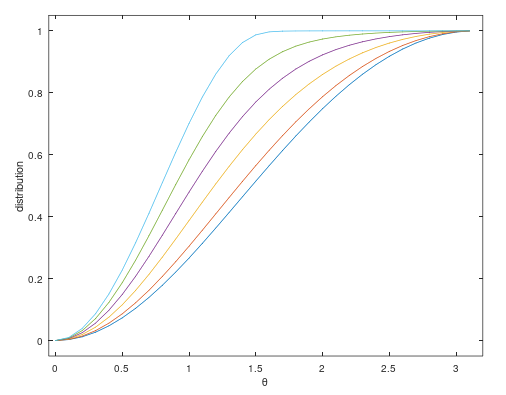
\includegraphics[width=10cm]{chapter_04_paragraph_16_exercice_2a}
		\caption{Exemples de distribution pour diff\'erentes valeurs de $\frac{V}{v_{0}}$, de 0.1 à 0.99, par int\'egration de l'\'equation (\ref{EQ:16_EX2A})}\label{FIG:4_16_EX2}
	\end{center}
\end{figure}

\subsubsection{$v_{0} < V$}

Dans ce cas, la m\^eme s\'equence calculatoire am\`ene \`a \'ecrire pour $\theta \in [0;\theta_{max}]$ :
\be
	\begin{Bmatrix}\dfrac{\mathrm{d}\omega_{0}}{4\pi}\end{Bmatrix}_{2} = \dfrac{1}{2}\sin\theta\left[2\dfrac{V}{v_{0}}\cos\theta - \dfrac{1 + \dfrac{V^{2}}{v_{0}^{2}}\cos(2\theta)}{\sqrt{1 - \dfrac{V^{2}}{v_{0}^{2}}\sin^{2}\theta}}\right]\mathrm{d}\theta
\ee
sachant qu'il faut prendre cette fois-ci dans l'\'equation (\ref{EQ:16_6}) les deux solutions, celles avec le signe - et celle avec le signe +, d\'eduite pr\'ec\`edemment. Ainsi la distribution totale pour $v_{0} < V$ s'obtient en faisant :
\be
	\begin{Bmatrix}\dfrac{\mathrm{d}\omega_{0}}{4\pi}\end{Bmatrix}_{1} - \begin{Bmatrix}\dfrac{\mathrm{d}\omega_{0}}{4\pi}\end{Bmatrix}_{2} = \dfrac{1 + \dfrac{V^{2}}{v_{0}^{2}}\cos(2\theta)}{\sqrt{1 - \dfrac{V^{2}}{v_{0}^{2}}\sin^{2}\theta}}\sin\theta\mathrm{d}\theta\label{EQ:16_EX2B}
\ee

\subsection{Intervalles angulaires dans <<~l~>>}